\documentclass[aspectratio=169]{beamer}

\usepackage[utf8]{inputenc}

\usepackage{amsmath}
\usepackage{graphicx}
\usepackage[T1]{fontenc}
\usepackage{siunitx}
\usepackage{libertine}
%\usepackage{libertinust1math}
%\usepackage[adobe-utopia]{mathdesign}
%\usepackage{wasysym}

% \usepackage{enumitem}
% \setitemize{label=\usebeamerfont*{itemize item}%
%   \usebeamercolor[fg]{itemize item}
%   \usebeamertemplate{itemize item},
% }%itemsep=\fill}
\setbeamertemplate{itemize item}[square]
\setbeamertemplate{itemize subitem}[circle]

\usepackage{pgfplots}
\pgfplotsset{compat=1.12}
\usepackage{tikz}
 \usetikzlibrary{arrows,decorations.pathmorphing,through,backgrounds,positioning,fit,petri}
 \usetikzlibrary{shapes,shadows}
 \usetikzlibrary{shapes.multipart}
 \usetikzlibrary{calc}
 \usetikzlibrary{decorations.pathreplacing}
 \usetikzlibrary{plotmarks}
\usepgfplotslibrary{fillbetween}


\tikzset{
	invisible/.style={opacity=0},
	visible on/.style={alt={#1{}{invisible}}},
	alt/.code args={<#1>#2#3}{%
		\alt<#1>{\pgfkeysalso{#2}}{\pgfkeysalso{#3}} % \pgfkeysalso doesn't change the path
	},
}

%\pgfplotsset{every axis/.append style={label style={font=\small},tick label style={font=\footnotesize} }}

% \definecolor{azulcito}{RGB}{20,70,140}
\definecolor{azulcito}{RGB}{80,80,140}
\definecolor{verdecito}{RGB}{0,128,128}
\definecolor{rojito}{RGB}{140,80,80}

\setbeamercolor*{structure}{fg=verdecito,bg=verdecito!20!white}
\setbeamercolor*{alerted text}{fg=verdecito}


  \setbeamercolor{block title}{fg=verdecito,bg=verdecito!20!white}%�
  \setbeamercolor{block body}{fg=black,bg=verdecito!10!white}
  
\beamertemplatenavigationsymbolsempty

\setbeamercolor*{author in head/foot}{fg=verdecito,bg=verdecito!20!white}
\setbeamercolor*{title in head/foot}{fg=verdecito,bg=verdecito!20!white}
\setbeamercolor*{date in head/foot}{fg=verdecito,bg=verdecito!20!white}

\newcommand{\graphheight}{6cm}
\newcommand{\graphwidth}{10cm}

\newtheorem{proposition}{Proposition}

\defbeamertemplate*{footline}{mitema}
{
  \leavevmode%
  \hbox{%
  \begin{beamercolorbox}[wd=.25\paperwidth,ht=2.25ex,dp=1ex,left]{author in head/foot}%
    \usebeamerfont{author in head/foot}\hspace*{2ex}\insertshortauthor
  \end{beamercolorbox}%
  \begin{beamercolorbox}[wd=.5\paperwidth,ht=2.25ex,dp=1ex,center]{title in head/foot}%
    \usebeamerfont{date in head/foot}\insertshortdate{}
  \end{beamercolorbox}%
  \begin{beamercolorbox}[wd=.25\paperwidth,ht=2.25ex,dp=1ex,right]{date in head/foot}%
    \insertframenumber{}/\inserttotalframenumber\hspace*{2em} 
  \end{beamercolorbox}}%
 \vskip0pt%
}


\setbeamercolor{blocky}{fg=verdecito,bg=verdecito!20!white}
\setbeamercolor{blocky2}{fg=black,bg=verdecito!10!white}

\defbeamertemplate*{title page}{customized}[1][]
{
{\flushright
  \begin{beamercolorbox}[wd=\paperwidth,right,rightskip=1.5em, sep=1em]{blocky}%
    \usebeamerfont{title}{\huge\inserttitle}\par %\vspace{.9em}
    \usebeamerfont{subtitle}{\Large \insertsubtitle}\par
  \end{beamercolorbox}%
  \vfill
    \usebeamerfont{author}{\Large \insertauthor}\par \vspace{1em}
      \usebeamerfont{institute}{\large \insertinstitute}\par
  
  
  \vfill
  \usebeamerfont{date}{\insertdate}\par
  \vfill
  \usebeamercolor[fg]{titlegraphic}\inserttitlegraphic
  }
}

\usefonttheme[onlymath]{serif}

\title{Spatial estimation of EV energy demand based on aggregated measurements}
 
\author[Andres Ferragut, Universidad ORT Uruguay]{\alert{Andres Ferragut}, Emiliano Espindola}
\institute{Universidad ORT Uruguay}
\date[INFORMS APS 2023]{INFORMS APS 2023 -- Nancy, France -- June 2023}
%\titlegraphic{\flushright\includegraphics[width=5em]{figuras/espindola.png} \large Joint work with Emiliano Espíndola}
%\setbeamertemplate{items}{$\blacksquare$ \hspace{.5em}}
%\AtBeginSection[]
%{
%\begin{frame}{Outline}
%\tableofcontents[currentsection, 
%    hideallsubsections, 
%    sectionstyle=show/shaded,
%]
%\end{frame}
%}


%\newtheorem{lemma}{Lemma}
%\newtheorem{theorem}{Theorem}
%\newtheorem{proposition}{Proposition}


%%%for better items
% \makeatletter
% \renewcommand{\itemize}[1][]{%
% 	\beamer@ifempty{#1}{}{\def\beamer@defaultospec{#1}}%
% 	\ifnum \@itemdepth >2\relax\@toodeep\else
% 	\advance\@itemdepth\@ne
% 	\beamer@computepref\@itemdepth% sets \beameritemnestingprefix
% 	\usebeamerfont{itemize/enumerate \beameritemnestingprefix body}%
% 	\usebeamercolor[fg]{itemize/enumerate \beameritemnestingprefix body}%
% 	\usebeamertemplate{itemize/enumerate \beameritemnestingprefix body begin}%
% 	\list
% 	{\usebeamertemplate{itemize \beameritemnestingprefix item}}
% 	{\def\makelabel##1{%
% 			{%
% 				\hss\llap{{%
% 						\usebeamerfont*{itemize \beameritemnestingprefix item}%
% 						\usebeamercolor[fg]{itemize \beameritemnestingprefix item}##1}}%
% 			}%
% 		}%
% 	}
% 	\fi%
% 	\setlength\itemsep{\fill}
% 	\ifnum \@itemdepth >1
% 	\vfill
% 	\fi%  
% 	\beamer@cramped%
% 	\raggedright%
% 	\beamer@firstlineitemizeunskip%
% }
% \def\enditemize{\ifhmode\unskip\fi\endlist%
% 	\usebeamertemplate{itemize/enumerate \beameritemnestingprefix body end}
% 	\ifnum \@itemdepth >1
% 	\vfil
% 	\fi%  
% }
% \makeatother
% %%%%

\begin{document}

\frame[plain]{\titlepage}

\begin{frame}{Introduction}

	\begin{itemize}
		\item Electrical vehicle (EV) adoption is currently growing exponentially.
		\item Less carbon emissions, noise and other efficiency benefits.
	\end{itemize}

	\vfill
	\alert{Problems:}
	\vfill
	\begin{itemize}
		\item We need to \alert{build the charging infrastructure} to replace gas stations.
		\item Charging is \alert{power and energy intensive} for the network, the grid must cope with the enlarged demand.
	\end{itemize}
	\vfill
	\pause
	
	\begin{center}
		\Large\alert{We need good spatial estimates of energy demand!}
	\end{center}
\end{frame}

\begin{frame}{Outline of the talk}
    \tableofcontents[hideallsubsections]
\end{frame}

% \AtBeginSection{%
% \begin{frame}{Outline of the talk}
%     \tableofcontents[currentsection]
% \end{frame}
% }

\section{Problem description}

\begin{frame}{The Problem}

	\begin{itemize}
		\item We need an \alert{spatial estimate} of energy demand in order to upgrade the distribution network.
		\item Currently, we do not have \alert{measurements} of this demand due to low EV penetration.
	\end{itemize}

	\vfill

	\begin{block}{Idea:}
		Use current \alert{gas consumption}, measured at gas stations, converted to energy.
	\end{block}

	\uncover<2->{
	\begin{block}{Challenge:}
		These measurements are \alert{concentrated} at the gas stations. How to interpolate them?
	\end{block}
	}

\end{frame}

\begin{frame}{Energy density}

	\vfill
	\begin{columns}
		\begin{column}{0.5\textwidth}
	
			\begin{itemize}
				\item We have an unkonwn \alert{energy density} $g(x)$ (in energy/\si{km^2}) over a region $\mathcal{X}$.
				
				\vspace{1cm}
				\item Represents amount of energy demand coming from a small ball around $x$.
			
			\end{itemize}
	
		\end{column}
		\begin{column}{0.5\textwidth}
			\centering
			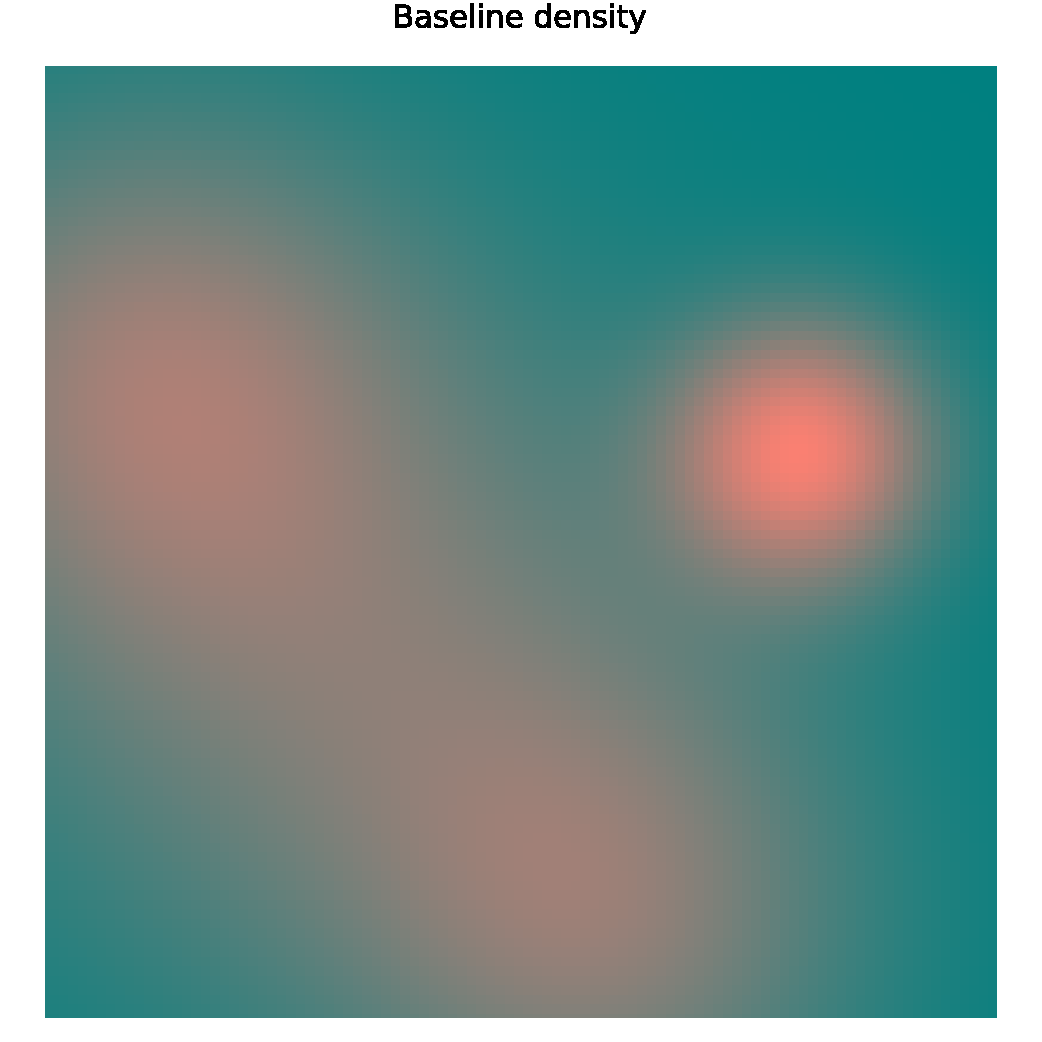
\includegraphics[width=0.9\columnwidth]{figuras/baseline_density.pdf}
		\end{column}
	\end{columns}
\end{frame}

\begin{frame}{Measurement points}

	\vfill
	\begin{columns}
		\begin{column}{0.5\textwidth}
			\begin{itemize}
				\item We cannot sample from this density!
				\vspace{1cm}
				\item All we have is some \alert{measurement points} distributed over $\mathcal{X}$.
				\vspace{1cm}
				\item What we can measure is the total demand coming from a cell around our measurement point.
			\end{itemize}
		\end{column}
		\begin{column}{0.5\textwidth}
			\centering
			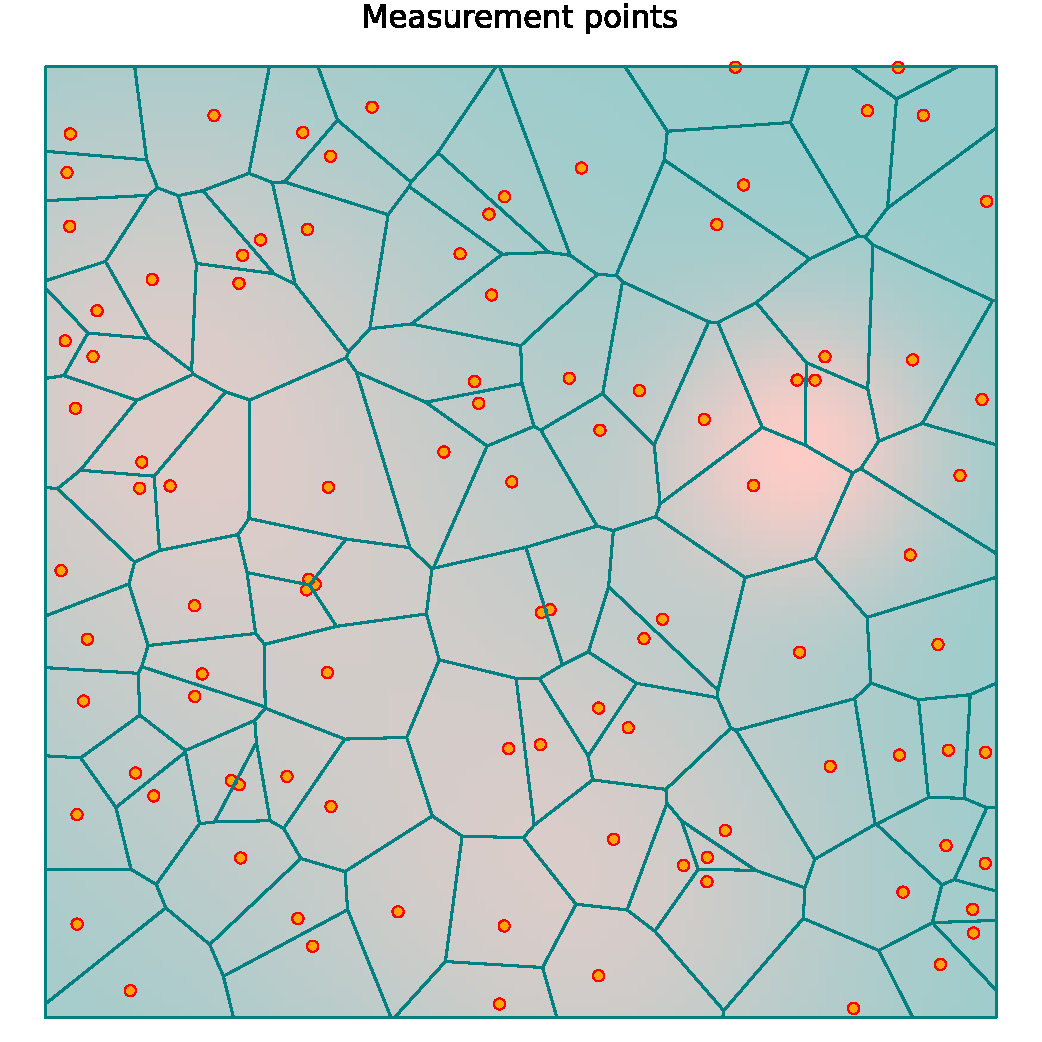
\includegraphics[width=0.9\columnwidth]{figuras/measurement_points.pdf}
		\end{column}
	\end{columns}

\end{frame}


\begin{frame}{Our dataset}
	\begin{columns}
		\begin{column}{0.5\textwidth}
			\begin{itemize}
				\item Each demand is measured at sites $s_i$.
				\vspace{1cm}
				\item We have access to $y_i = \int_{V_i} g(x)dx$, where $V_i$ is the Voronoi cell of site $i$.
				\vspace{1cm}
				\item The size of the circle represents measured demand at the sites.
			\end{itemize}
		\end{column}
		\begin{column}{0.5\textwidth}
			\centering
			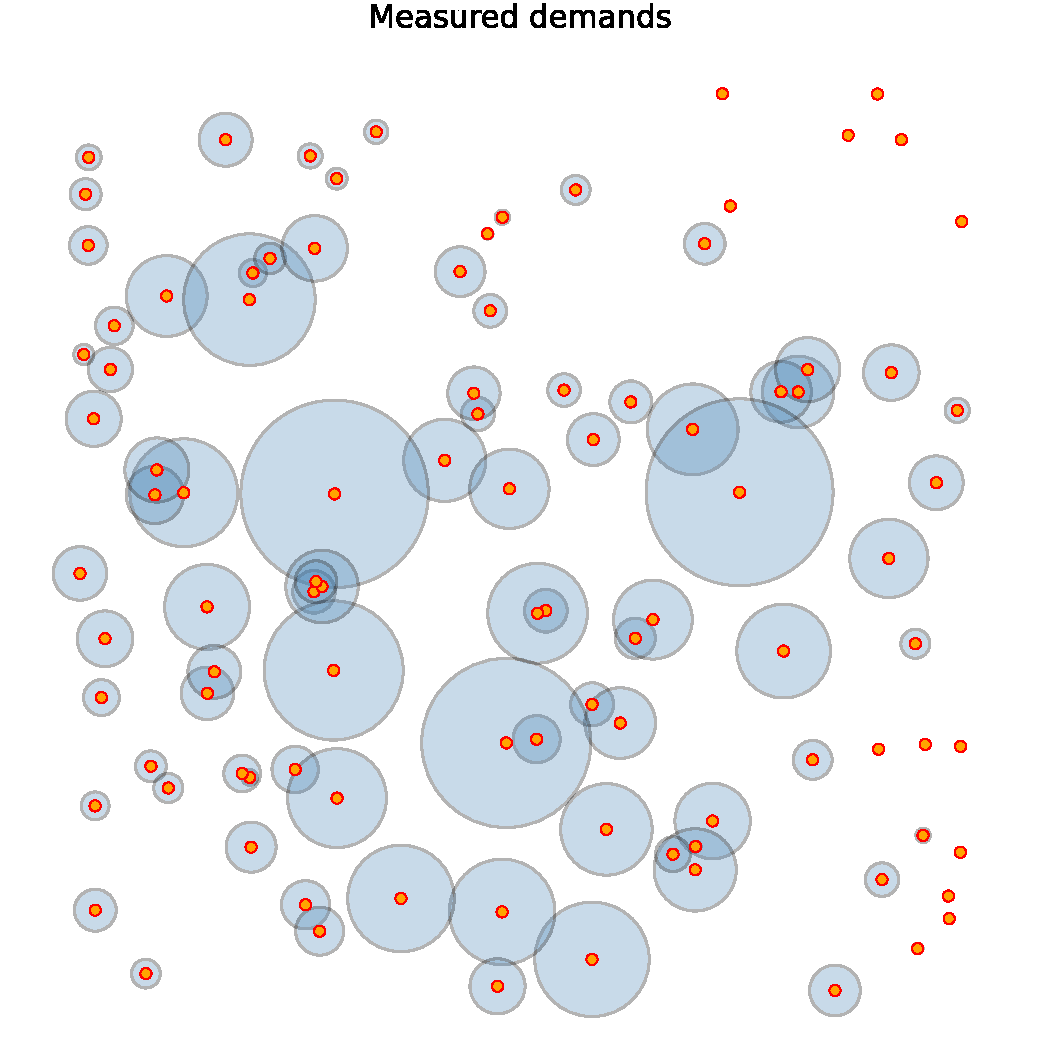
\includegraphics[width=0.9\columnwidth]{figuras/measured_demands.pdf}
		\end{column}
	\end{columns}

\end{frame}

\begin{frame}{Mathematical formulation}

	\begin{itemize}
		\item In a region of space $\mathcal{X}\subset \mathbb{R}^d$, we are given:
		\vspace{0.5cm}
		\begin{itemize}
			\item A list of \alert{fixed} sites $\{s_1,\ldots,s_m\}$, $s_i\in \mathcal{X}$.
			\vspace{0.5cm}

			\item A list of measurements $\{y_1,\ldots,y_m\}$, $y_i\geqslant 0$.
		\end{itemize}
\vfill
		\item \alert{Goal:} construct an estimate $\hat{g}(x;\theta)$ of the spatial density such that:
		\begin{equation*}
			\int_{V_i} g(x;\theta) \,dx \approx y_i \quad \forall i
		\end{equation*}
		where $V_i$ is a \alert{cell} associated with site $s_i$ (e.g. the Voronoi cell).
	\end{itemize}
\end{frame}


\begin{frame}{Non-parametric approach}{Not very fun...and maybe useless}
	
	\begin{columns}
		\begin{column}{0.5\textwidth}
			\begin{itemize}
				\item First approach: \alert{histogram counts}.
				\vspace{0.5cm}
				\item Estimate
				
				 \begin{equation*}
					g_H(x) = \sum_{i} \frac{y_i}{\mathrm{m}(V_i)} \mathbf{1}_{V_i}(x)
				 \end{equation*}
				\vspace{0.5cm}
				\item Non-smooth. Low interpolation properties. Not suitable for low-dimensional representation.
			\end{itemize}
		\end{column}
		\begin{column}{0.5\textwidth}
			\centering
			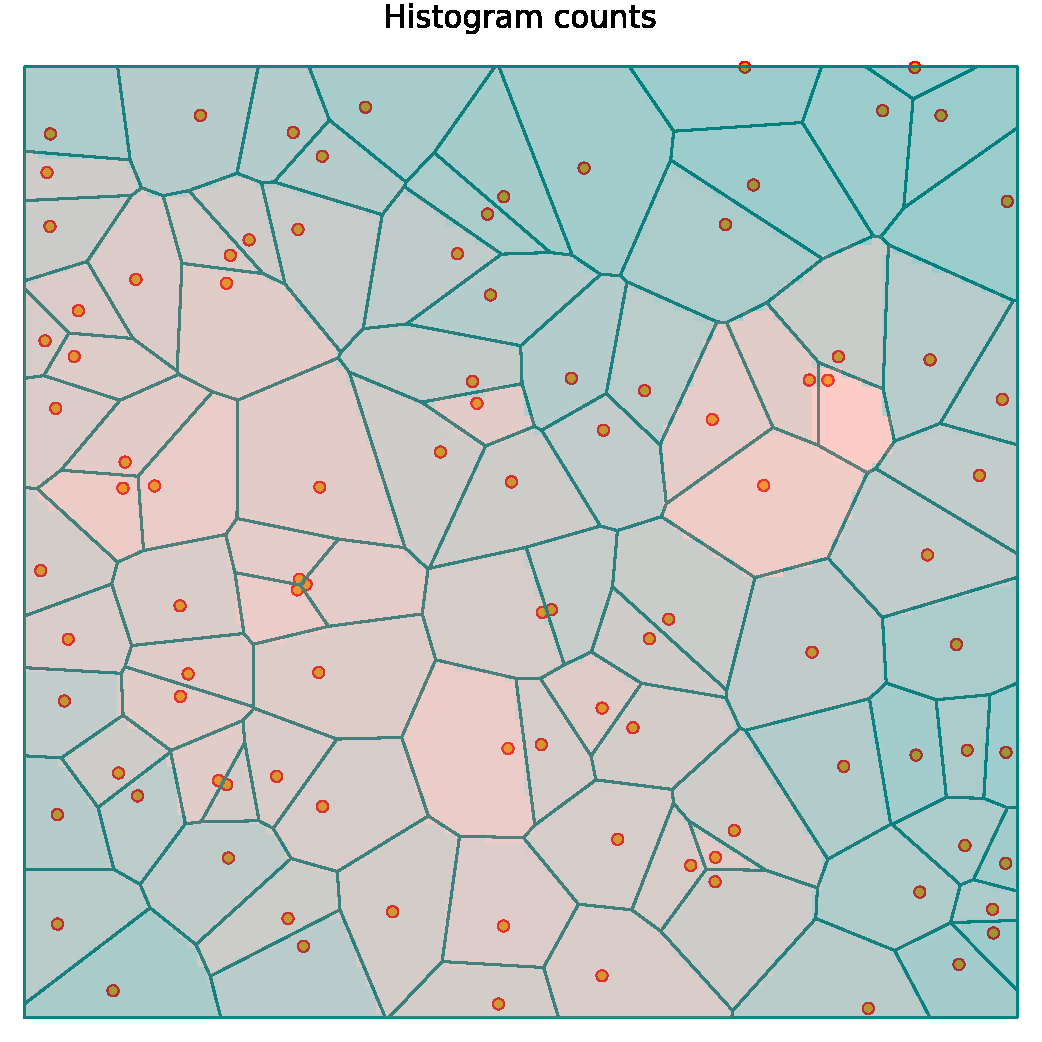
\includegraphics[width=0.9\columnwidth]{figuras/histogram_counts.pdf}
		\end{column}
	\end{columns}


\end{frame}

\section{Radial basis functions approach}

\begin{frame}{Radial basis functions}
	
	To obtain a lower dimensional representation we use \alert{radial basis functions} to estimate $g(x)$. Namely, our estimator has the form:

	\begin{equation*}
		g_{RBF} (x;\theta) = \sum_{j=1}^n w_j e^{-\frac{||x-\mu_j||^2}{2\sigma_j^2}}
	\end{equation*}
	where $\theta = (\{w_j\},\{\mu_j\},\{\sigma_j^2\})$.

	\vfill

	\begin{itemize}
		\item $w_j\in\mathbb{R^+}$ are the \alert{weights}, 
		\item $\mu_j\in\mathbb{R}^d$ are the \alert{nodes} and 
		\item $\sigma_j^2\in\mathbb{R}^+$ the \alert{bandwidths}.
	\end{itemize}


\end{frame}

\begin{frame}{Least squares approach}

	\begin{itemize}

		\item Since we have access to the cell measurements, it makes sense to consider the loss function:
		\begin{equation*}
			L(\theta) = \frac{1}{2}\sum_{i=1}^m \left(\int_{V_i} g_{RBF}(x;\theta) dx - y_i\right)^2
		\end{equation*}

		\item Therefore, the least squares estimator becomes:

		\begin{equation*}
			\hat{\theta}_{LS} = \arg\min_{\theta} L(\theta)
		\end{equation*}

		\item We now show an algorithm to compute this estimator.
	\end{itemize}
	
\end{frame}

\begin{frame}{Computing the weights}

	Consider first given the nodes $\mu_j$ and the bandwidths $\sigma_j^2$, we have:

	\begin{equation*}
		\int_{V_i} g_{RBF}(x,\theta)dx = \sum_{j=1}^n w_j \int_{V_i} e^{-\frac{||x-\mu_j||^2}{2\sigma_j^2}} dx =: \sum_{j=1}^n a_{ij}w_j.
	\end{equation*}
	The loss becomes:
	\begin{equation*}
		L(\theta) = \frac{1}{2}\sum_{i=1}^m \left(\sum_{j=1}^n a_{ij}w_j - y_i\right)^2 = \frac{1}{2}||Aw-y||^2
	\end{equation*}
	And thus we have the linear least squares problem:
	\begin{equation*}
		\min \frac{1}{2}||Aw-y||^2, \quad s.t. \; w\geqslant 0.
	\end{equation*}

	It can be readily solved, typically the constraint is not active.
\end{frame}

\begin{frame}{Estimating nodes and bandwidths}

	\begin{itemize}
		\item To estimate ${\mu_j}$ and $\{\sigma_j^2\}$ we may use \alert{gradient descent}. Note that:
		\begin{equation*}
			\frac{\partial L}{\partial \theta_k} = \sum_{i=1}^m \left(\int_{V_i} g_{RBF}(x;\theta) dx - y_i\right) \left(\int_{V_i} \frac{\partial}{\partial \theta_k}g_{RBF}(x;\theta) dx\right)
		\end{equation*}
		\vfill
		\item Moreover, due to the structure of the RBF functions:
		\begin{eqnarray*}
			\frac{\partial}{\partial \mu_j}g_{RBF}(x;\theta) &= \left[\frac{x-\mu_j}{\sigma_j^2}\right] w_j e^{-\frac{||x-\mu_j||^2}{2\sigma_j^2}} \\
			\frac{\partial}{\partial \sigma_j^2}g_{RBF}(x;\theta) &= \left[\frac{||x-\mu_j||^2}{2(\sigma_j^2)^2}\right] w_je^{-\frac{||x-\mu_j||^2}{2\sigma_j^2}}
		\end{eqnarray*}
	\end{itemize}		


\end{frame}
	

\begin{frame}{Computing the gradient}


So in order to compute the gradient, we need to estimate the following \alert{moments} of our current density estiamte:

\begin{equation*}
	\int_{V_i} g_{RBF}(x,\theta) \, dx, \quad \int_{V_i} \left[\frac{x-\mu_j}{\sigma_j^2}\right] g_{RBF}(x,\theta) \,dx, \quad \int_{V_i} \left[\frac{||x-\mu_j||^2}{2(\sigma_j^2)^2}\right] g_{RBF}(x,\theta) \,dx.
\end{equation*}
for each cell $i$.
\end{frame}

\begin{frame}{Estimating the moment integrals}{Monte Carlo approach}

	Sample $N$ uniformly distributed points in the region $\mathcal{X}$ and estimate:
	\begin{equation*}
		\int_{V_i} g_{RBF}(x;\theta)dx \approx \frac{\mathrm{m}(\mathcal{X})}{N}\sum_{k=1}^N g_{RBF}(u_k;\theta)\mathbf{1}_{V_i}(u_k)
	\end{equation*}
\pause
	\alert{Two possible variants:}

	\begin{itemize}
		\item Use a large $N$ and fix the estimation points $\to$ slightly more bias, less variance, faster to compute.
		\item Resample a relatively small $N$ on each step $\to$ less bias, high variance, amounts to Stochastic Gradient Descent.
	\end{itemize}
\end{frame}
	
\begin{frame}{Algorithm}{Stochastic gradient descent version}

	Given a suitable initial condition $\theta^{(0)} = (\{w_j^{(0)}\},\{\mu_j^{(0)}\},\{{\sigma_j^2}^{(0)}\})$, at each step $k$:

	\vfill 
	\begin{enumerate}
		\item Sample $N$ uniformly distributed random points in $\mathcal{X}$.
		\item Estimate the moment integrals and compute the gradient $\nabla L(\theta^{(k)})$.
		\item Perform a gradient step:
		\begin{equation*}
		\mu_j \leftarrow \mu_j - \alpha_k 	\nabla L(\theta^{(k)})_{\mu_j}, \quad \sigma_j^2 \leftarrow \sigma_j^2 - \alpha_k 	\nabla L(\theta^{(k)})_{\sigma_j^2}.
		\end{equation*}
		with step size $\alpha_k \sim O(1/k)$.
		\item For the new nodes and bandwidths, recompute $w_j$ using linear least squares.
		\item Update $\theta^{(k+1)}$ and iterate until convergence.
	\end{enumerate}
\end{frame}

\begin{frame}{Choosing the initial condition}

	We need a good first estimate $\theta^{(0)}$. We propose the following method: 

	\vfill

	\alert{Bootstrapping:}

	Fix the number of kernels $n$ as an hyperparameter and do:
	\vfill
	\begin{enumerate}
		\item Given the sites $\{s_1,\ldots,s_m\}$ and the measurements $\{y_1,\ldots,y_m\}$, run \alert{weighted $k-$means} with $n$ clusters to optimize:
		\begin{equation*}
			\min_{\mu_j} \sum_{j=1}^n \sum_{i \text{ closest to } \mu_j} y_i ||s_i-\mu_j||^2
		\end{equation*}

		\item Estimate the bandwidths $\sigma_j^2$ as the mean square distance of the allocated sites to node $j$.
		
		\item Compute a first estimate of $w_j$ by solving the linear least squares problem with the above initial estimates.
	\end{enumerate}
\end{frame}

\begin{frame}{Example: reconstructing the original density}{Initial condition}


	\begin{columns}
		
		\begin{column}{0.5\textwidth}
			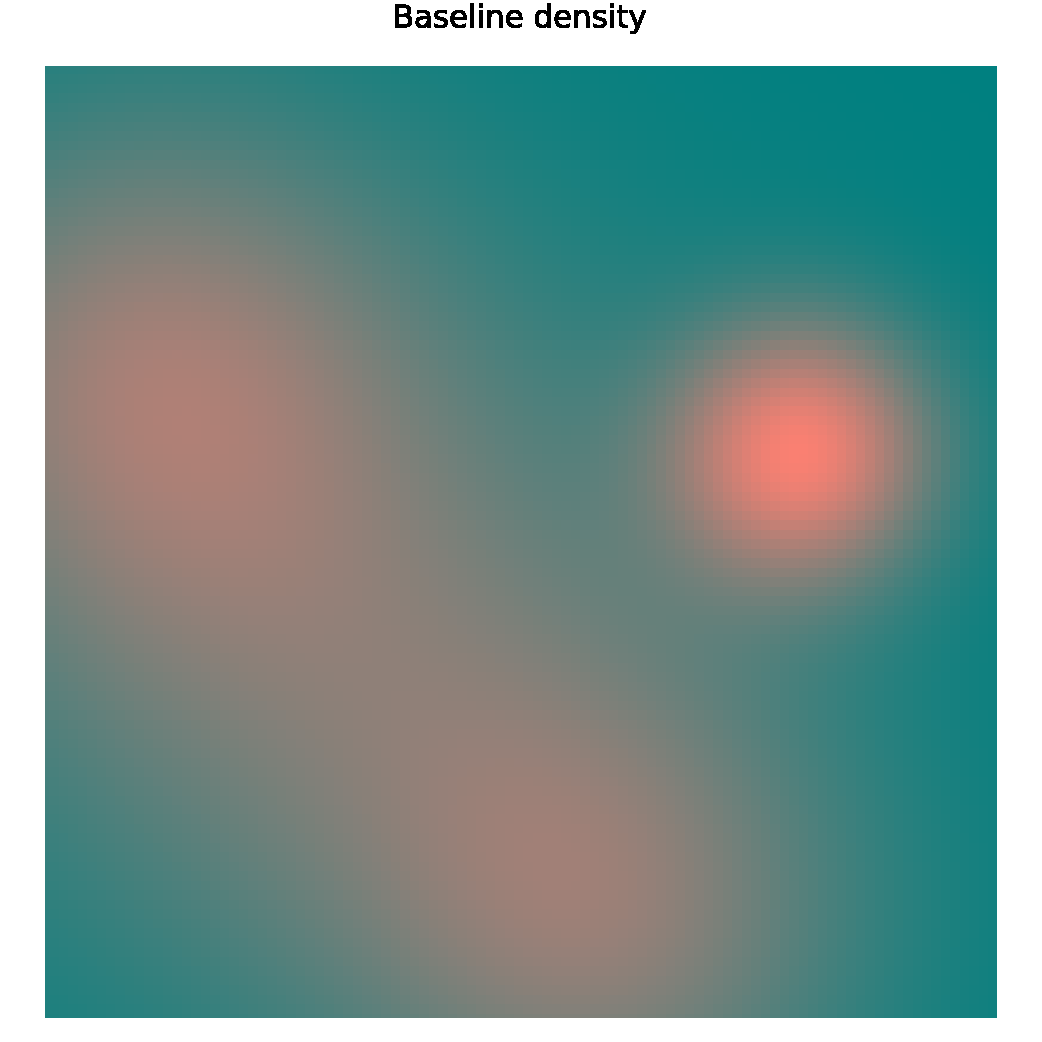
\includegraphics[width=\columnwidth]{figuras/baseline_density.pdf}
		\end{column}
		\begin{column}{0.5\textwidth}
			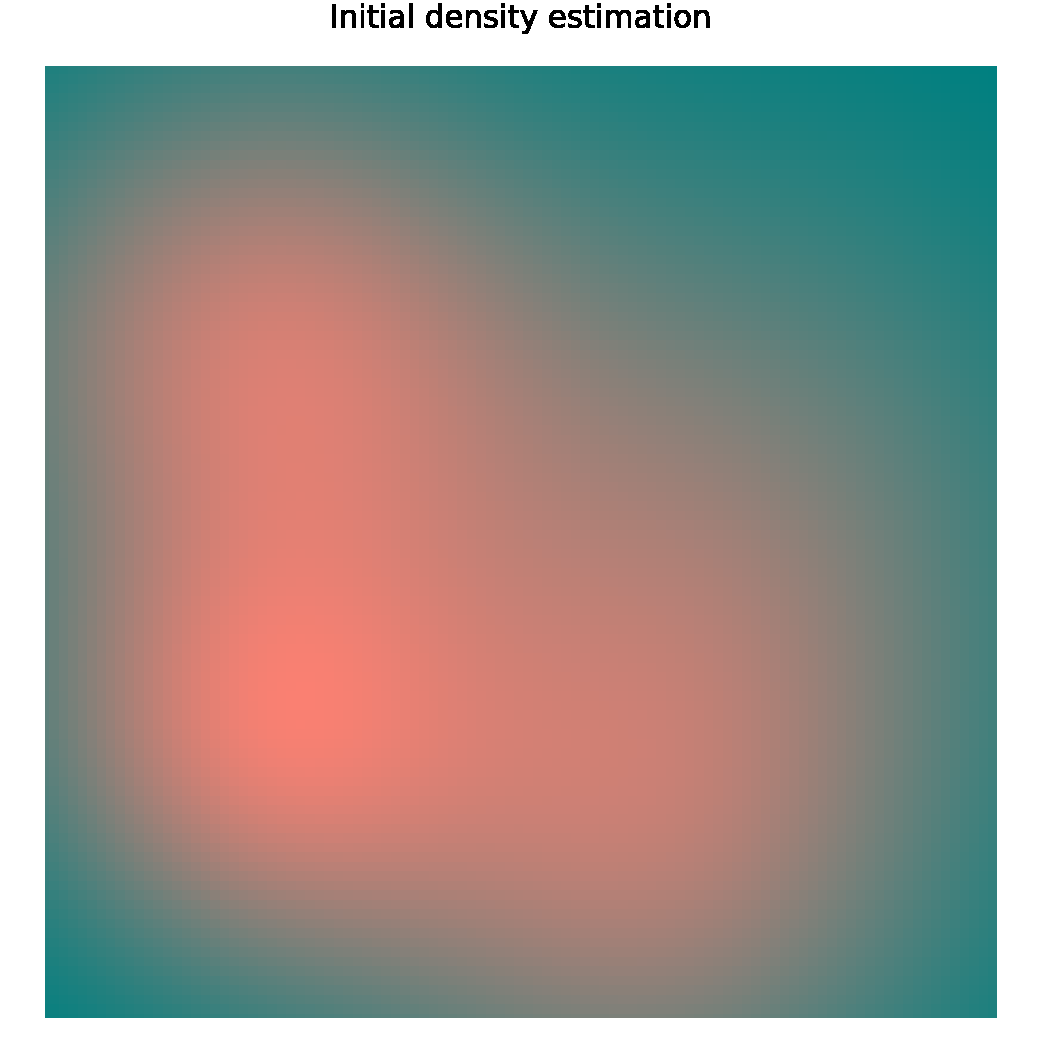
\includegraphics[width=\columnwidth]{figuras/initial_condition.pdf}			
		\end{column}

	\end{columns}

\end{frame}

\begin{frame}{Example: reconstructing the original density}{Root mean square loss evolution:}

	\begin{center}
		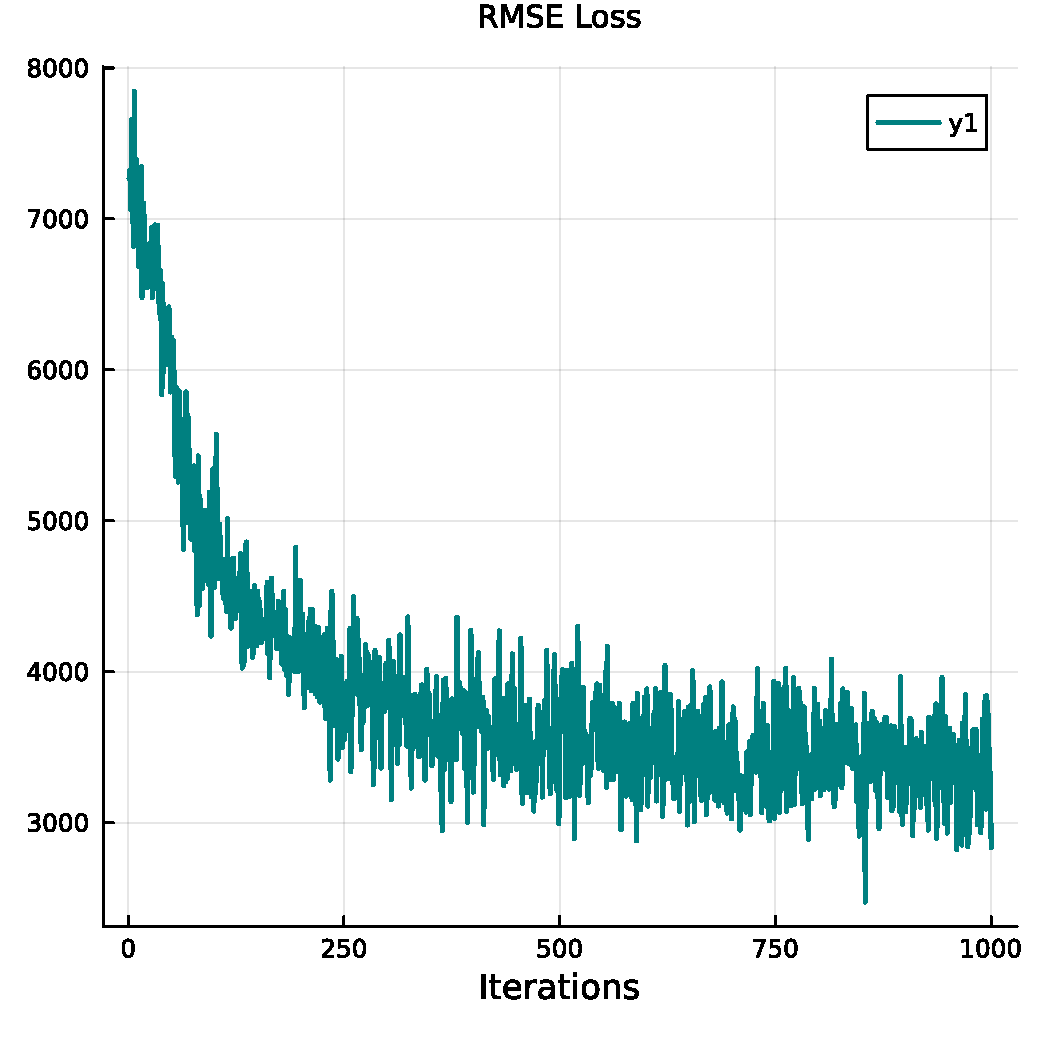
\includegraphics[width=0.45\textwidth]{figuras/rmse_loss.pdf}
	\end{center}		
		
\end{frame}

\begin{frame}{Example: reconstructing the original density}{Final estimate:}

	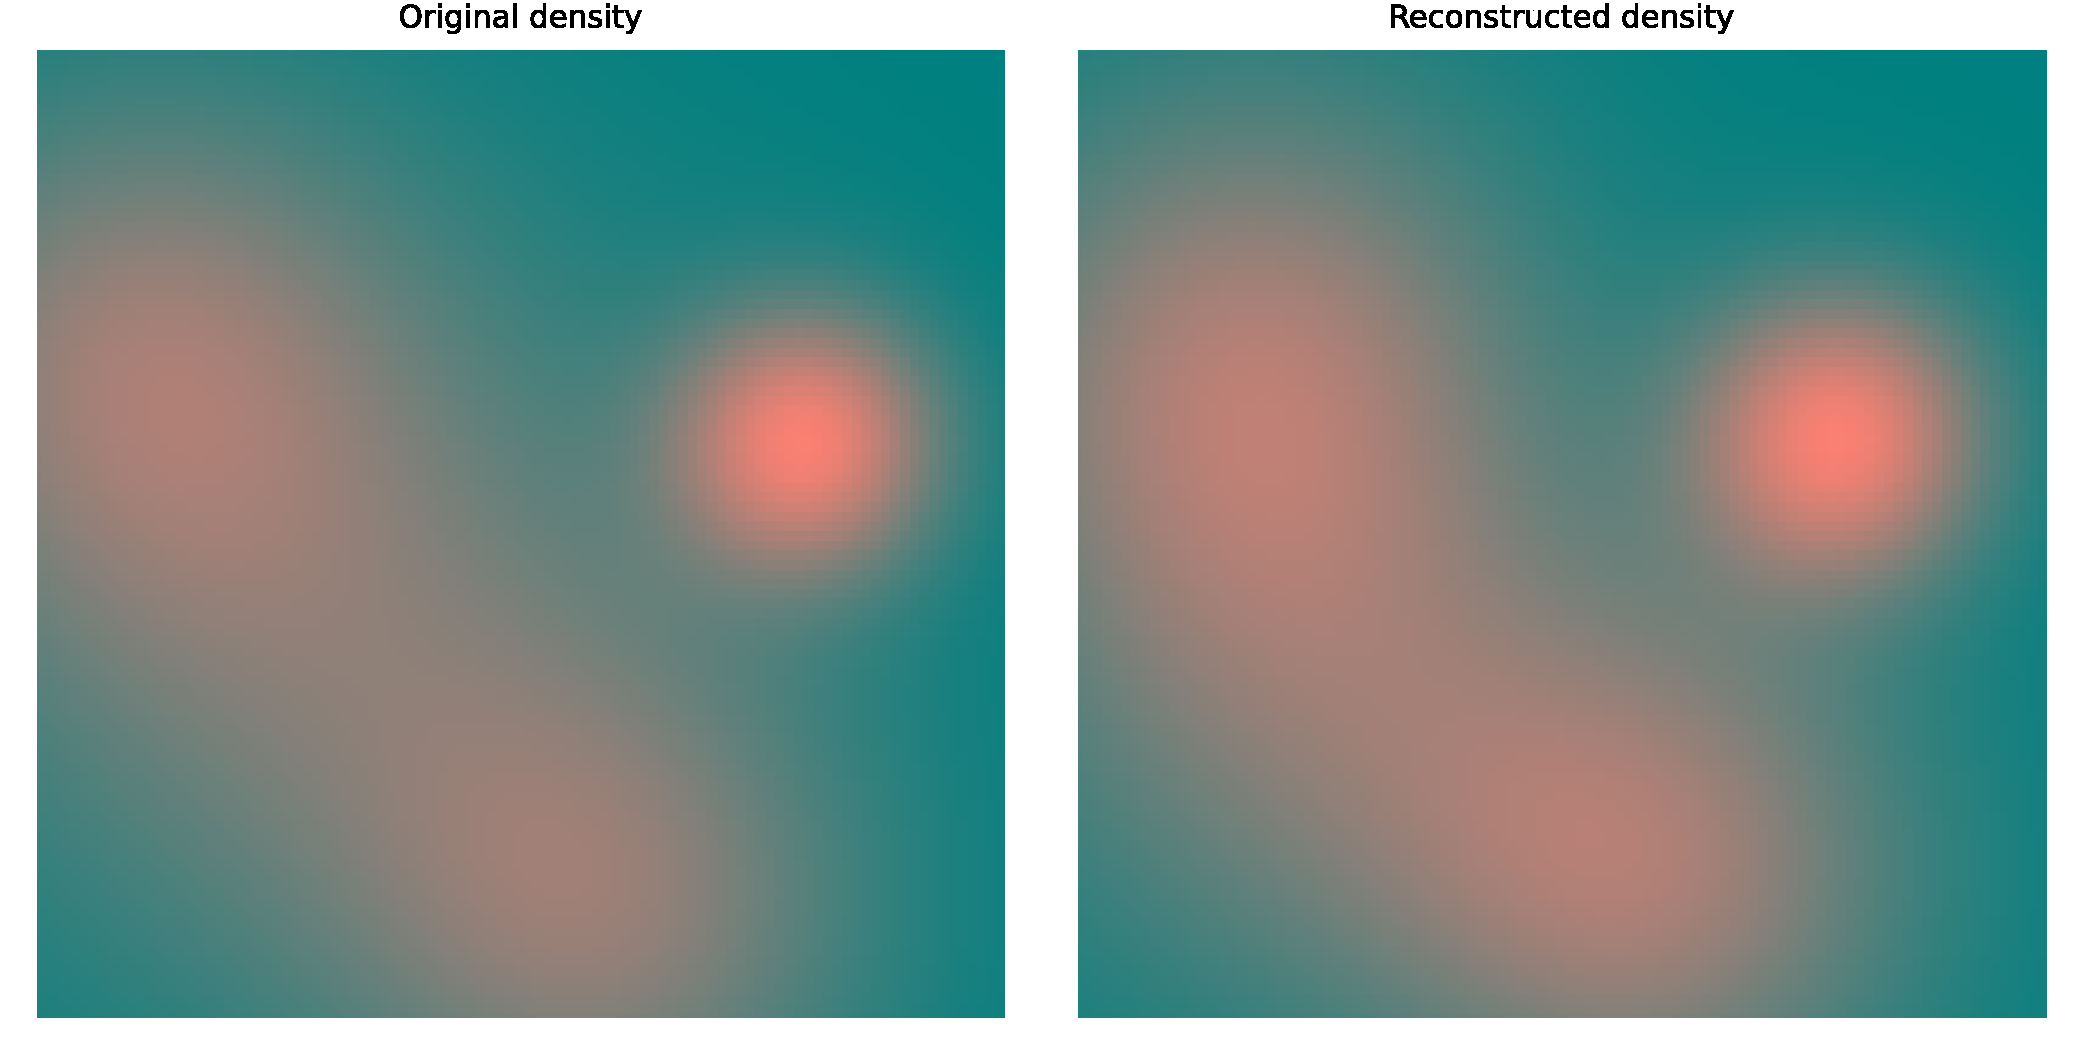
\includegraphics[width=\columnwidth]{figuras/least_squares_result.pdf}			

\end{frame}

\section{A Poisson parametric model}

\begin{frame}{Hidden Poisson process parametric model}

	Assume now that demands come from a \alert{marked Poisson process} 
	$$\Phi=\sum \delta_{(x_k,v_k)}$$ with:
	\vfill
	\begin{itemize}
		\item Spatial intensity $\Lambda(dx)$, $x\in\mathcal{X}$, modeled through an RBF density $\lambda(x;\theta)dx$.
		\vfill
		\item Individual marks (customer demands) exponentially distributed with rate $\nu$.
	\end{itemize}
	
\end{frame}

\begin{frame}{Hidden Poisson process parametric model}{Example}

	A realization of the process $\Phi$:

	\begin{columns}
		
		\begin{column}{0.5\textwidth}
			\centering
			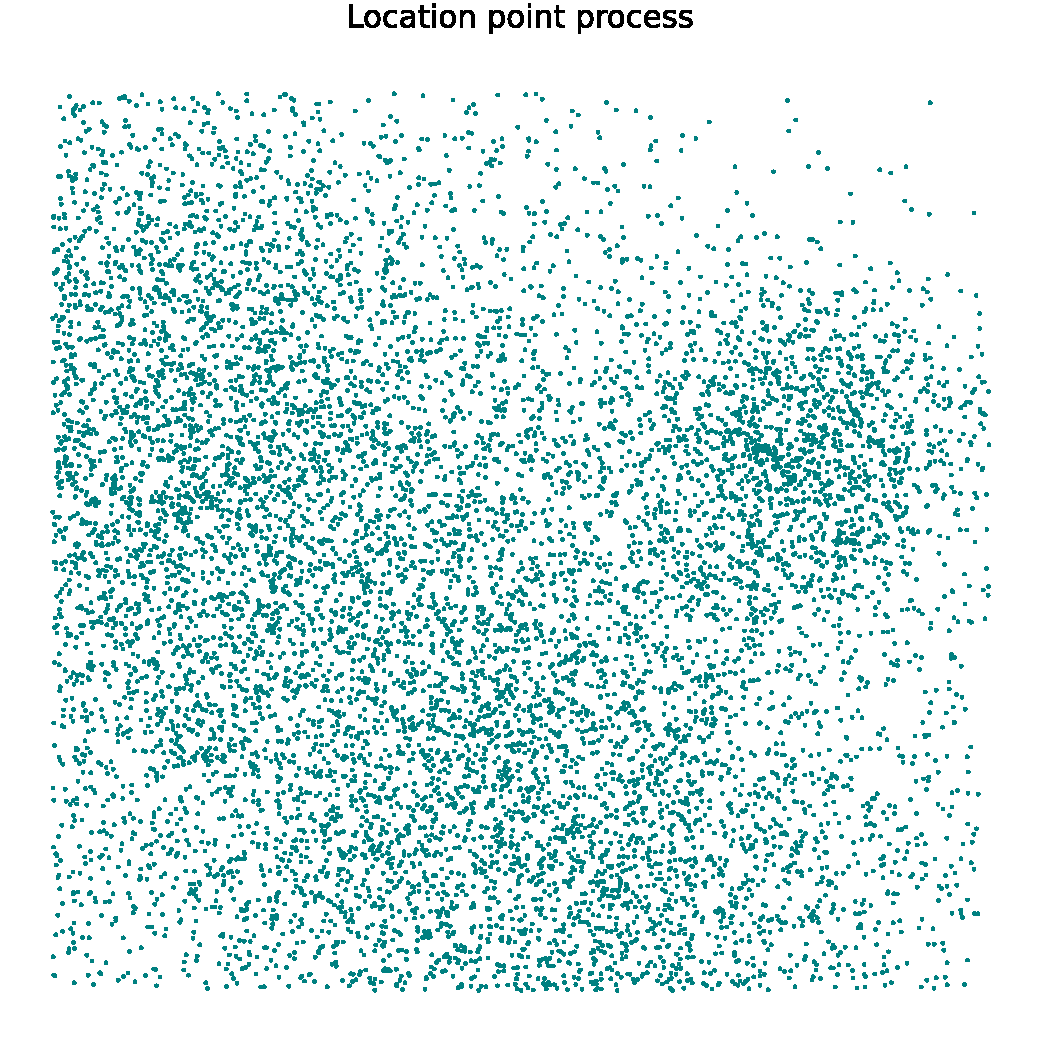
\includegraphics[width=0.8\columnwidth]{figuras/location_process.pdf}
		\end{column}
		\begin{column}{0.5\textwidth}
			\centering
			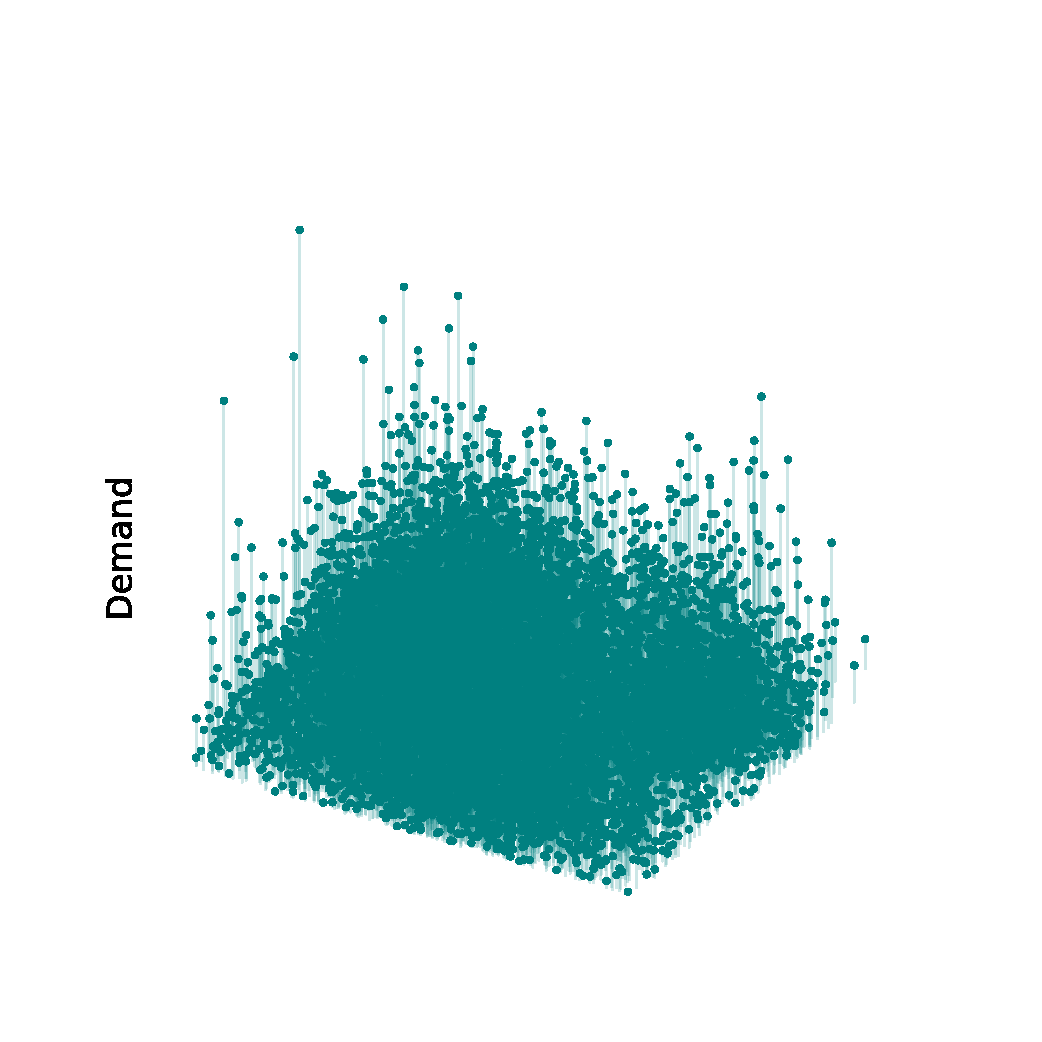
\includegraphics[width=\columnwidth]{figuras/location_and_demand.pdf}			
		\end{column}

	\end{columns}


\end{frame}

\begin{frame}{Observation model}

	\begin{columns}
		
		\begin{column}{0.5\textwidth}
			\begin{itemize}
				\item We observe the total cell demands:
					\begin{equation*}
						Y_i = \int_{V_i} v \,\Phi(dx,dv) = \sum_{k} v_k \mathbf{1}_{\{x_k\in V_i\}}
					\end{equation*}

				\item For each cell:
				\begin{eqnarray*}
					N_i \sim& \mathrm{Poisson}(\lambda_i(\theta))\\
					Y_i =& \sum_{k=1}^{N_i} V_k
				\end{eqnarray*}
				with $V_k\sim\exp(\nu)$ and cells are independent.
			\end{itemize}
		\end{column}

		\begin{column}{0.5\textwidth}
			\centering
			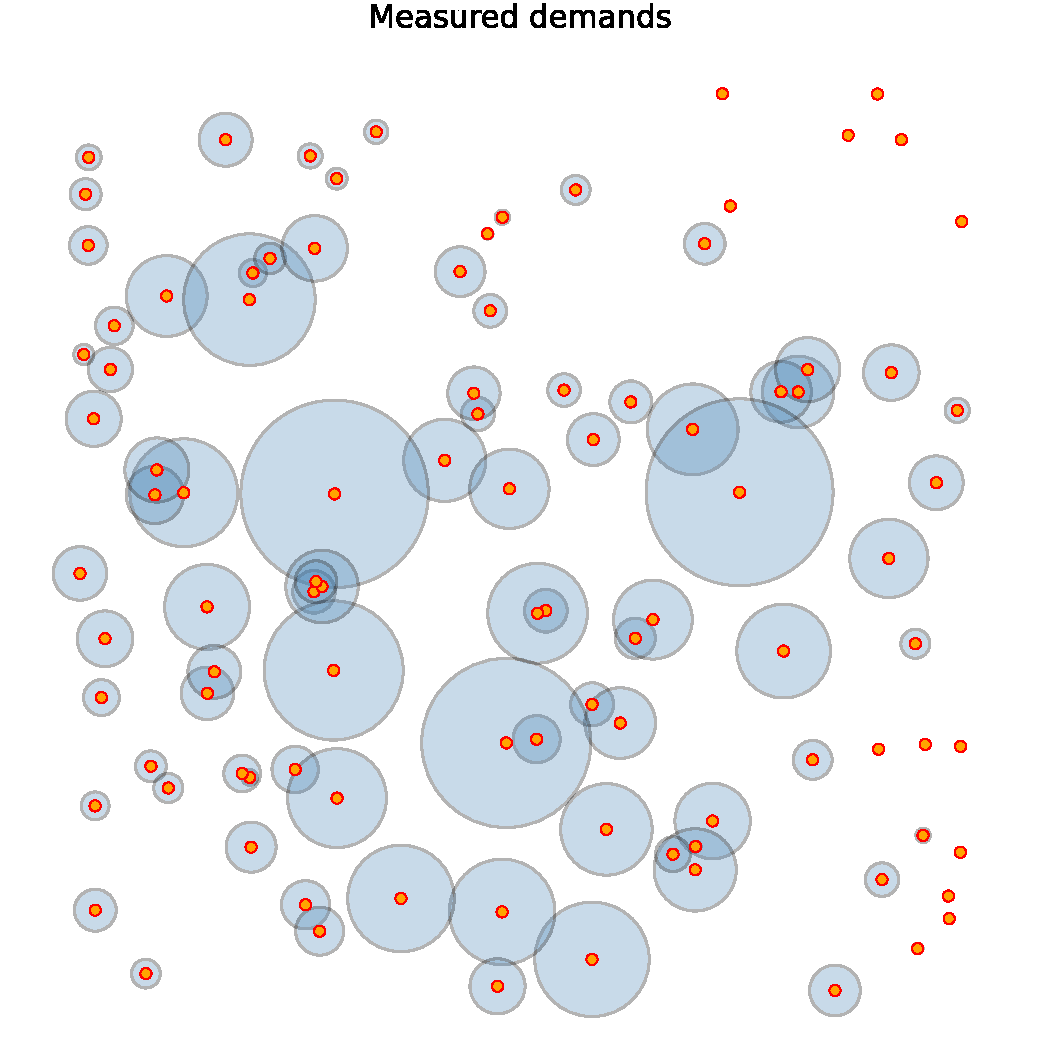
\includegraphics[width=0.9\columnwidth]{figuras/measured_demands.pdf}
		\end{column}
		
	\end{columns}
		\vfill


		\alert{Problem:} the number of points acts as a \emph{hidden variable}.

\end{frame}
	

\begin{frame}{Maximum likelihood approach}

	\begin{itemize}
		\item Ideally one would like to maximize $p(y;\theta)$. Difficult to compute.
		\item Expectation-Maximization approaches fail (a posteriori distribution also difficult).
		\item Consider maximizing the combined likelihood:
		\begin{equation*}
			p(n,y) = \prod_{i=1}^m e^{-\lambda_i(\theta)}\frac{\lambda_i(\theta)^{n_i}}{n_i!}p(y_i\mid n_i), \quad \text{with }\lambda_i(\theta) = \int_{V_i} \lambda(x;\theta)dx
		\end{equation*}
		\item Now, since given $n_i$, the demands are independent exponentials we have:
		\begin{equation*}
			p(y_i\mid n_i) = \frac{1}{(n_i-1)!}\nu^{n_i}y_i^{n_i-1}e^{-\nu y_i}.
		\end{equation*}
	\end{itemize}
\end{frame}

\begin{frame}{Maximizing the counts likelihood}

Given an estimate of $\Lambda(dx)$ and $\nu$, we can maximize \alert{each term} over $n_i$, thus decoding the hidden variable:

\begin{equation*}
	\max_{n_i} e^{-\lambda_i(\theta)}\frac{\lambda_i(\theta)^{n_i}}{n_i!} \frac{1}{(n_i-1)!}\nu^{n_i} y_i^{n_i-1}e^{-\nu y_i}.
\end{equation*}

The maximum is attained for:
\begin{equation*}
	n_i^*(n_i^*+1) = \lambda_i(\theta) \nu y_i
\end{equation*}

That is:
\begin{equation*}
	n_i^* \approx \sqrt{\lambda_i(\theta) \nu y_i}.
\end{equation*}
\end{frame}

\begin{frame}{Estimating the RBF parameters}


	With the hidden variables estimated, the joint likelihood as a function of $\theta$ is:
	\begin{equation*}
		\ell(\theta;n,y) = \sum_{i=1}^m -\lambda_i(\theta) + n_i\log(\lambda_i(\theta)) + n_i\log(\nu) - \nu y_i + (n_i-1)\log(y_i) - \log(n_i!(n_i-1)!).
	\end{equation*}
	
	The new estimate for $\nu$ follows immediately by differentiation:
	\begin{equation*}
		\hat{\nu} = \frac{\sum_i n_i}{\sum_i y_i}.
	\end{equation*}
	
	As for the RBF parameters, we perform a gradient approach as before:
	\begin{equation*}
	\frac{\partial \ell}{\partial \theta} = \sum_{i=1}^m \frac{\partial \ell}{\partial \lambda_i}\frac{\partial \lambda_i}{\partial \theta} = \sum_{i=1}^m \left[\frac{n_i}{\lambda_i(\theta)}-1\right]\frac{\partial \lambda_i(\theta)}{\partial \theta}.
	\end{equation*}
	The derivatives of $\lambda_i(\theta)$ are similar to the preceding ones.
\end{frame}

\begin{frame}{Maximum likelihood algorithm}

	Given a suitable initial condition $\theta^{(0)} = (\{w_j^{(0)}\},\{\mu_j^{(0)}\},\{{\sigma_j^2}^{(0)}\},\nu^{(0)})$, at each step $k$, iterate until convergence:

	\vfill 
	\begin{enumerate}
		\item Sample $N$ uniformly distributed random points in $\mathcal{X}$.
		\item Estimate $\lambda_i(\theta)$ ant the moment integrals to compute its gradient.
		\item Decode the hidden variables $n_i = \sqrt{\lambda_i(\theta^{(k)})\nu^{(k)}y_i}$
		\item Perform a gradient step on nodes and bandwidths:
		\begin{gather*}
			w_j^{(k+1)} = w_j^{(k+1)}+ \alpha_k 	\nabla \ell(\theta^{(k)})_{w_j},\\
		\mu_j^{(k+1)} = \mu_j^{(k)} + \alpha_k 	\nabla \ell(\theta^{(k)})_{\mu_j}, \quad (\sigma_j^2)^{(k+1)} \leftarrow (\sigma_j^2)^{(k)} + \alpha_k 	\nabla \ell(\theta^{(k)})_{\sigma_j^2}.
		\end{gather*}
		\item Update $\hat{\nu}^{(k+1)} = \frac{\sum_i n_i}{\sum_i y_i}$.
	\end{enumerate}
\end{frame}



\begin{frame}{Example}{Maximum likelihhod reconstruction}

			\centering
			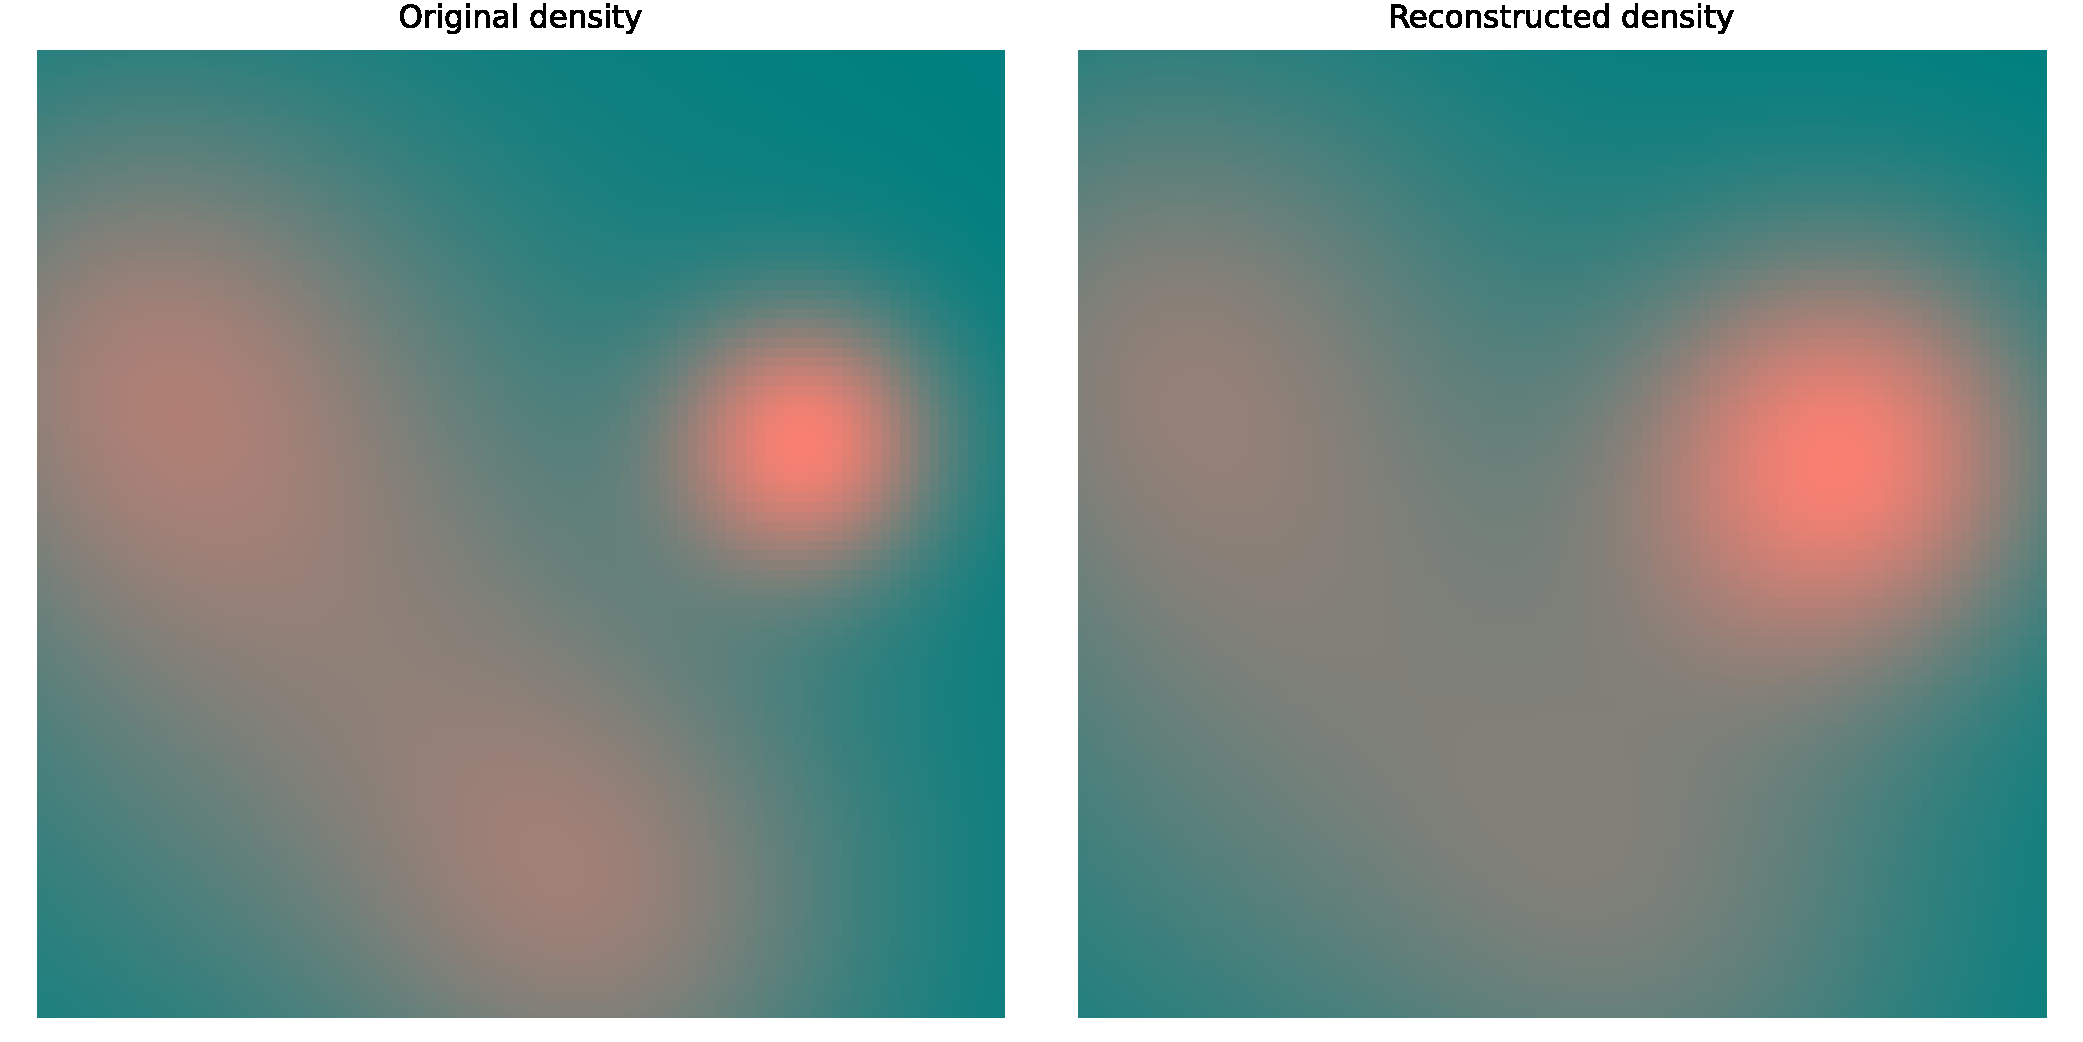
\includegraphics[width=0.9\columnwidth]{figuras/maximum_likelihood_reconstruction.pdf}

			
\end{frame}

\begin{frame}{Application}{Gas sales data from California}

	Annual consumption of gas in LAX aggregated by ZIP code:

	\vfill
\begin{columns}
	\begin{column}{0.33\textwidth}
		\centering
		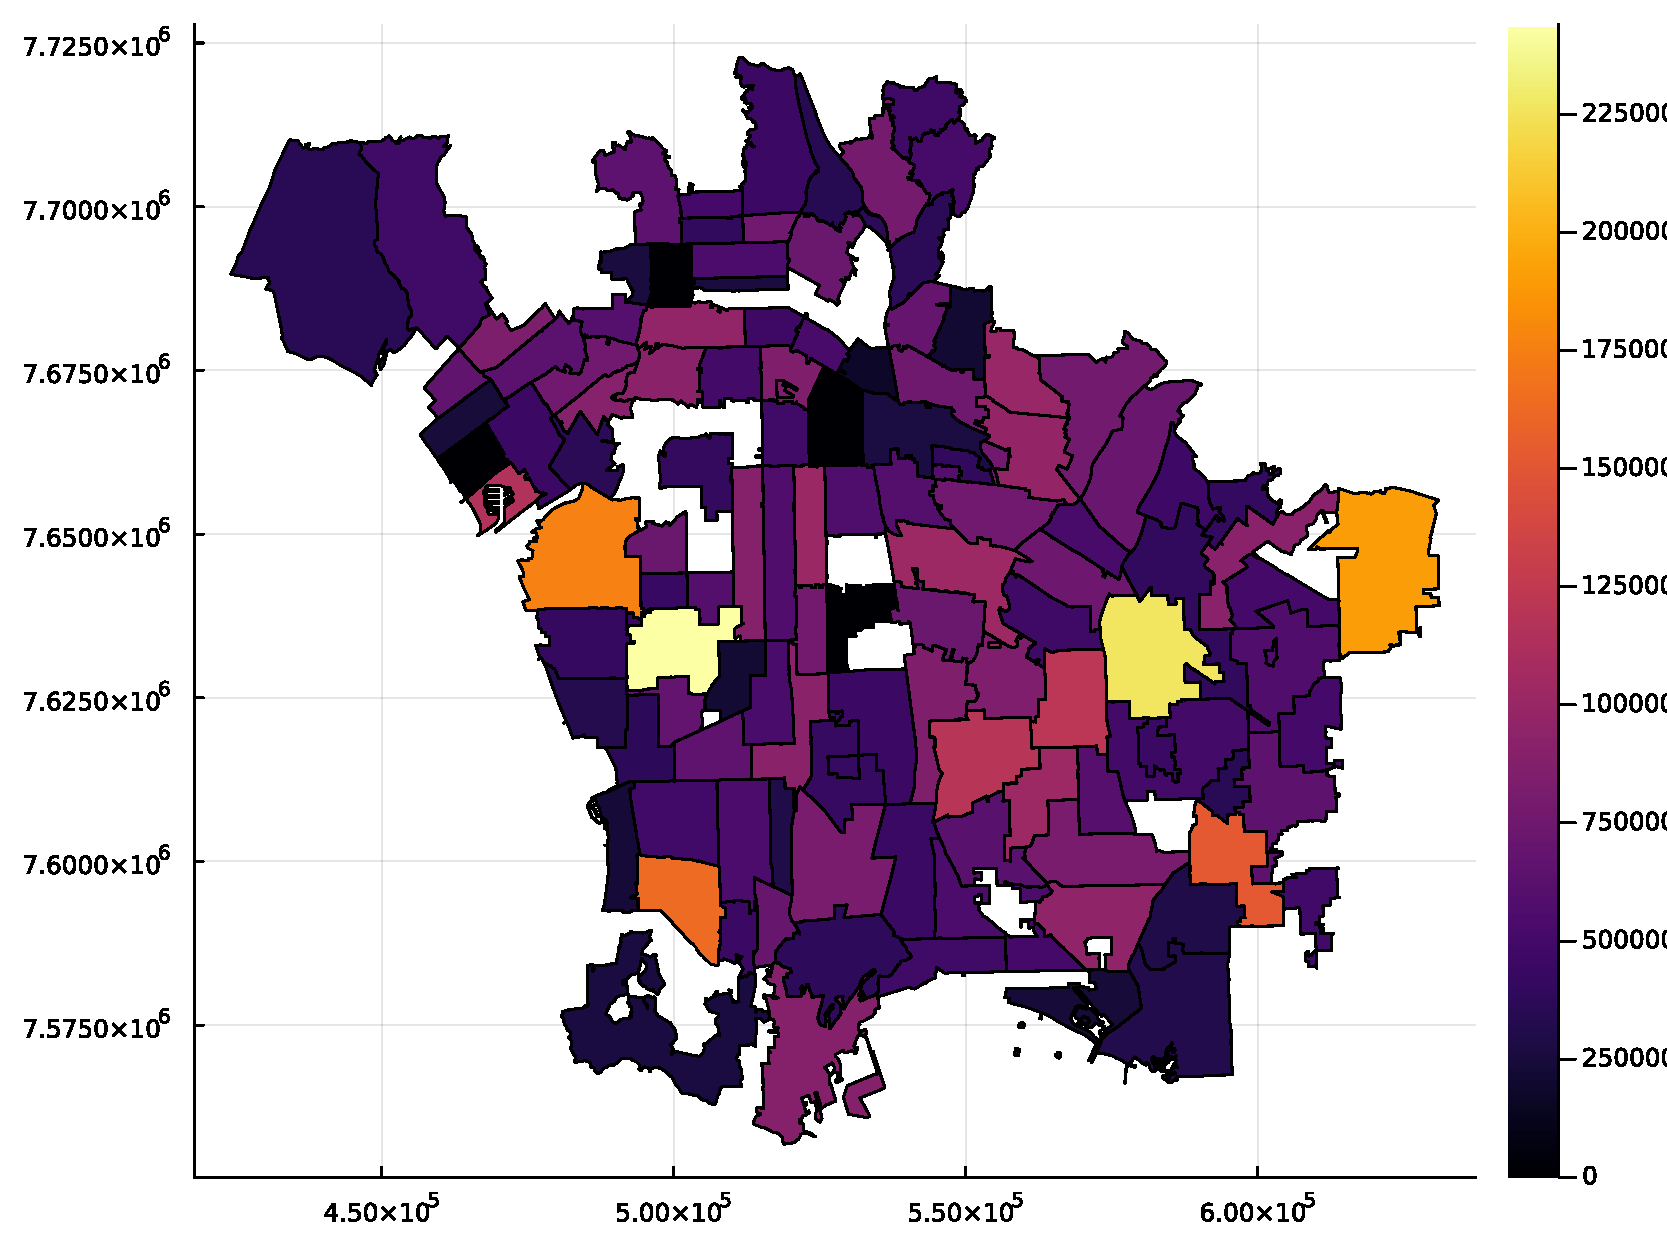
\includegraphics[width=\columnwidth]{figuras/real.pdf}		
	\end{column}
	\begin{column}{0.33\textwidth}
		\centering
		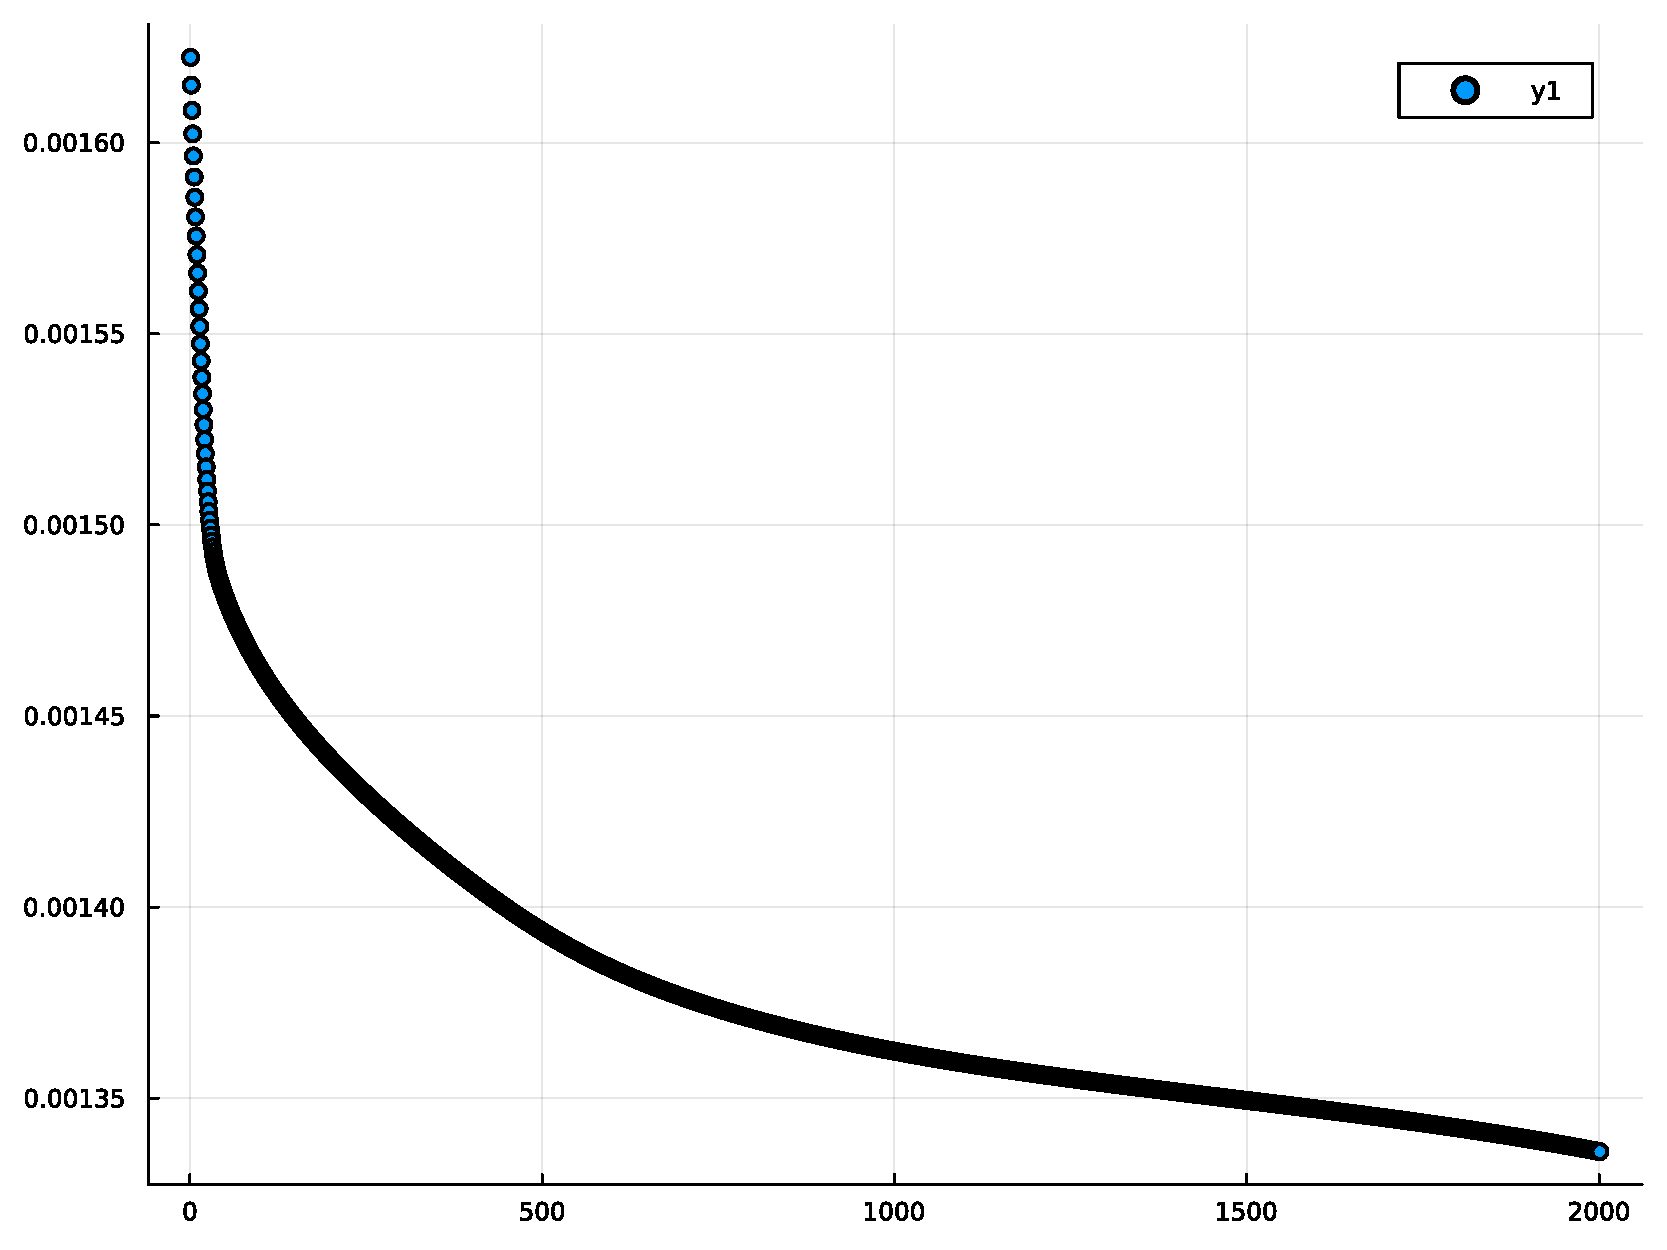
\includegraphics[width=\columnwidth]{figuras/loss.pdf}				
	\end{column}
	\begin{column}{0.33\textwidth}
		\centering
		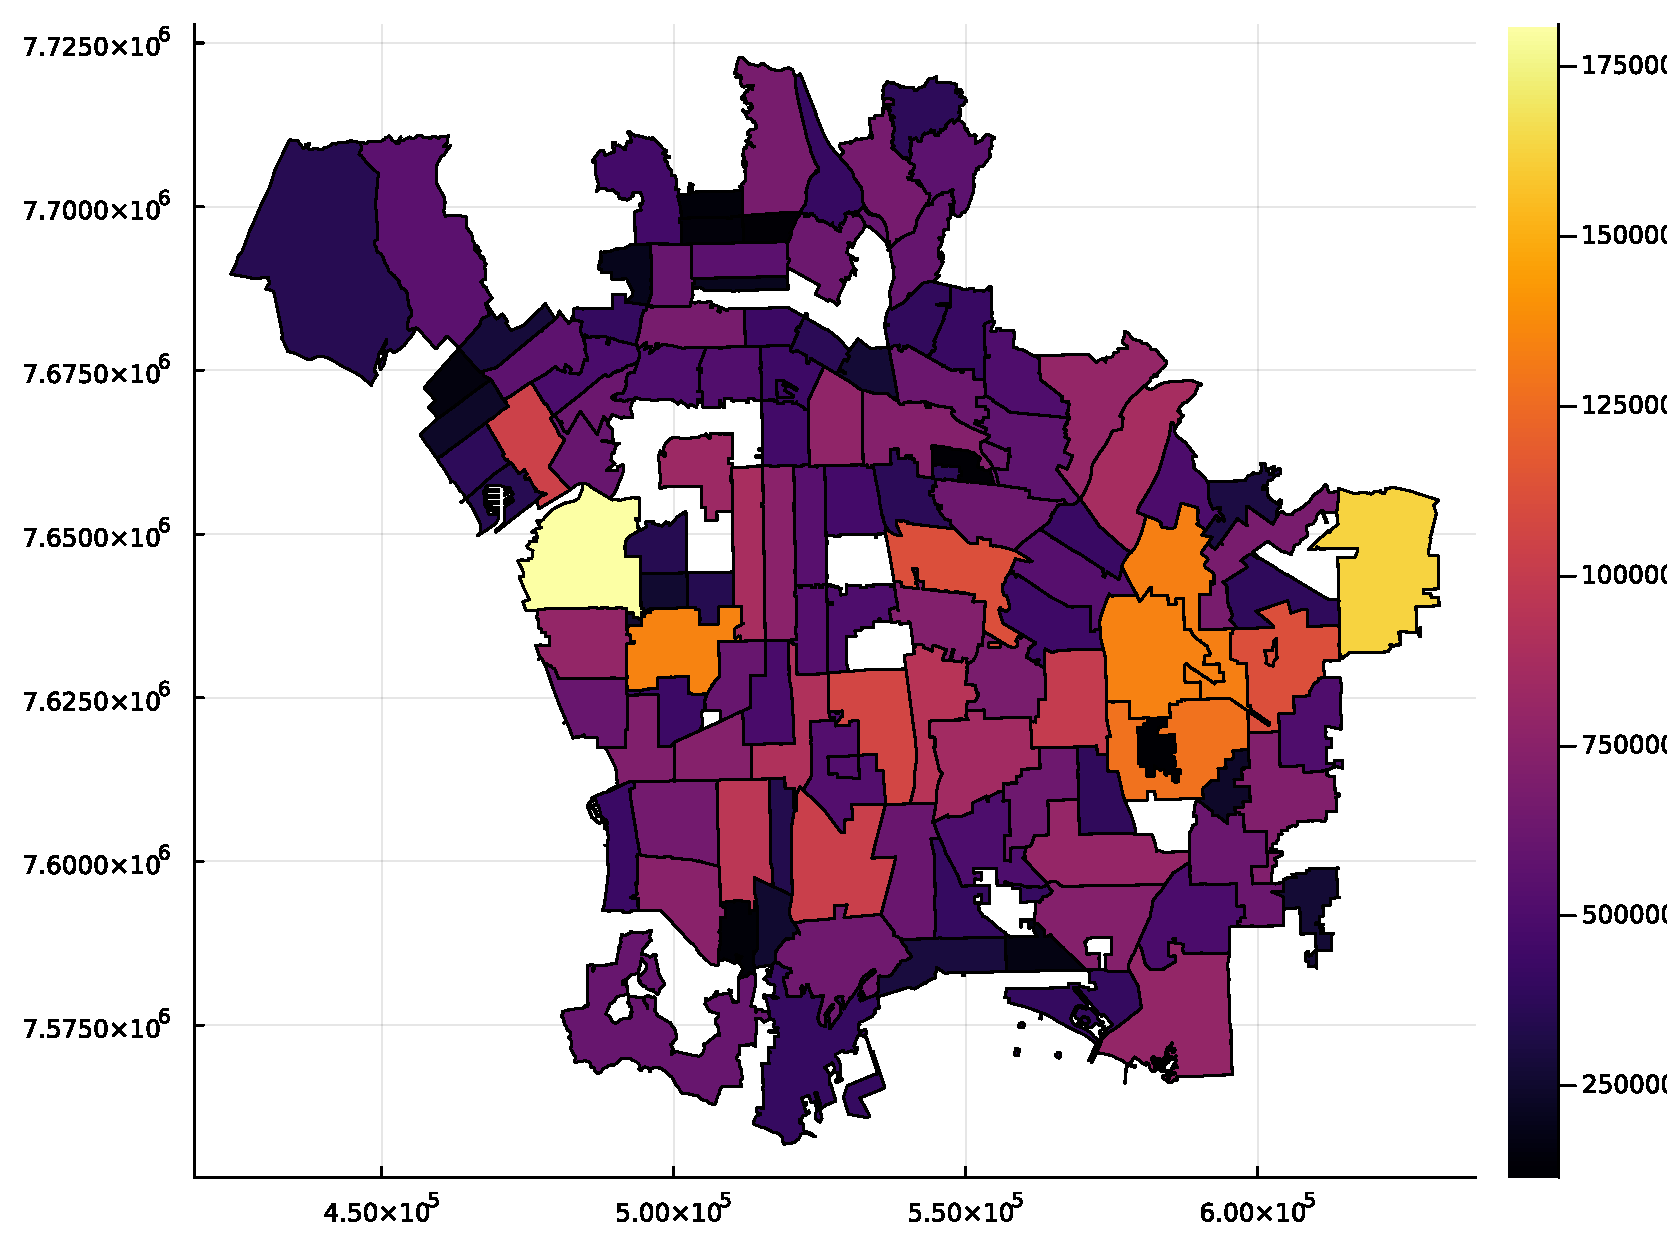
\includegraphics[width=\columnwidth]{figuras/estimated.pdf}		
	\end{column}

\end{columns}

\end{frame}

% \begin{frame}{Application}{Gas sales data from California}
	
% \end{frame}

\section{Final remarks}

\begin{frame}{Take home messages...}
\begin{itemize}
	\item EVs are popping up, we have to prepare the infrastructure.
	
	\vfill
	\item We can estimate spatial energy demand based on current gas consumption measurements.
	
	\vfill
	\item We analyzed two different approaches with different properties.
	
	\vfill
	\item We would like to expand on the mathematical analysis, in particular the connection with stochastic gradient descent and more general transport measures and problems.
\end{itemize}
\end{frame}

\begin{frame}[plain]
	
	
	\vfill
	
	{\Huge \alert{Thank you!}}
	
	% \vfill
	% 
	% {\Large For more details...}
	
	\vfill
	
	Andres Ferragut
	
	ferragut@ort.edu.uy
	
	\alert{http://aferragu.github.io}
	
	
\end{frame}

\end{document}
